%% abtex2-modelo-relatorio-tecnico.tex, v-1.7.1 laurocesar
%% Copyright 2012-2013 by abnTeX2 group at http://abntex2.googlecode.com/ 
%%
%% This work may be distributed and/or modified under the
%% conditions of the LaTeX Project Public License, either version 1.3
%% of this license or (at your option) any later version.
%% The latest version of this license is in
%%   http://www.latex-project.org/lppl.txt
%% and version 1.3 or later is part of all distributions of LaTeX
%% version 2005/12/01 or later.
%%
%% This work has the LPPL maintenance status `maintained'.
%% 
%% The Current Maintainer of this work is the abnTeX2 team, led
%% by Lauro César Araujo. Further information are available on 
%% http://abntex2.googlecode.com/
%%
%% This work consists of the files abntex2-modelo-relatorio-tecnico.tex,
%% abntex2-modelo-include-comandos and abntex2-modelo-references.bib
%%

% ------------------------------------------------------------------------
% ------------------------------------------------------------------------
% abnTeX2: Modelo de Relatório Técnico/Acadêmico em conformidade com 
% ABNT NBR 10719:2011 Informação e documentação - Relatório técnico e/ou
% científico - Apresentação
% ------------------------------------------------------------------------ 
% ------------------------------------------------------------------------

% Alterado por Rodrigo Campiolo para apresentação de relatórios na disciplina
% de Redes de Computadores II do Bacharelado em Ciência da Computação da UTFPR-CM.


\documentclass[
	% -- opções da classe memoir --
	12pt,				% tamanho da fonte
	%openright,			% capítulos começam em pág ímpar (insere página vazia caso preciso)
	oneside,   	        % para impressão em verso e anverso use twoside. Oposto a oneside
	a4paper,			% tamanho do papel. 
	% -- opções da classe abntex2 --
	%chapter=TITLE,		% títulos de capítulos convertidos em letras maiúsculas
	%section=TITLE,		% títulos de seções convertidos em letras maiúsculas
	%subsection=TITLE,	% títulos de subseções convertidos em letras maiúsculas
	%subsubsection=TITLE,% títulos de subsubseções convertidos em letras maiúsculas
	% -- opções do pacote babel --
	english,			% idioma adicional para hifenização
	french,				% idioma adicional para hifenização
	spanish,			% idioma adicional para hifenização
	brazil,				% o último idioma é o principal do documento
	]{pacotes/abntex2}


% ---
% PACOTES
% ---

% ---
% Pacotes fundamentais 
% ---
\usepackage{cmap}				% Mapear caracteres especiais no PDF
\usepackage{lmodern}			% Usa a fonte Latin Modern
\usepackage[T1]{fontenc}		% Selecao de codigos de fonte.
\usepackage[utf8]{inputenc}		% Codificacao do documento (conversão automática dos acentos)
\usepackage{indentfirst}		% Indenta o primeiro parágrafo de cada seção.
\usepackage{color}				% Controle das cores
\usepackage{graphicx}			% Inclusão de gráficos
% ---
\usepackage[utf8]{inputenc}

\usepackage{float}
% ---
% Pacotes adicionais, usados no anexo do modelo de folha de identificação
% ---
\usepackage{multicol}
\usepackage{multirow}
% ---
	
% ---
% Pacotes adicionais, usados apenas no âmbito do Modelo Canônico do abnteX2
% ---
\usepackage{lipsum}				% para geração de dummy text
% ---

% ---
% Pacotes de citações
% ---
\usepackage[brazilian,hyperpageref]{backref}	 % Paginas com as citações na bibl
\usepackage[alf]{pacotes/abntex2cite}	% Citações padrão ABNT
\usepackage{comment}
% --- 
% CONFIGURAÇÕES DE PACOTES
% --- 

% % ---
% % Configurações do pacote backref
% % Usado sem a opção hyperpageref de backref
% \renewcommand{\backrefpagesname}{Citado na(s) página(s):~}
% % Texto padrão antes do número das páginas
% \renewcommand{\backref}{}
% % Define os textos da citação
% \renewcommand*{\backrefalt}[4]{
% 	\ifcase #1 %
% 		Nenhuma citação no texto.%
% 	\or
% 		Citado na página #2.%
% 	\else
% 		Citado #1 vezes nas páginas #2.%
% 	\fi}%
% ---

% ---
% Informações de dados para CAPA e FOLHA DE ROSTO
% ---
\titulo{Atividade de Engenharia de Software - Requisitos (Parte 2)}
\autor{Igor Ortega Carmona RA: 00236524 \\ Victor Hugo Volpato de Almeida RA: 00136760 \\ Estudantes de Análise e Desenvolvimento de Sistemas (ADS) }
\local{Cianorte}
\data{Novembro / 2022}
\instituicao{%
  UNIPAR - CIANORTE
  \par
  Tecnologia em Análise e Desenvolvimento de Sistemas (ADS)
}
\tipotrabalho{Relatório técnico}
% O preambulo deve conter o tipo do trabalho, o objetivo, 
% o nome da instituição e a área de concentração 
\preambulo{Atividade avaliativa para a matéria de \textit{Engenharia de Software 1}, grade do curso de \textit{Análise e Desenvolvimento de Sistemas}. }
% ---

% ---
% Configurações de aparência do PDF final

% alterando o aspecto da cor azul
\definecolor{blue}{RGB}{41,5,195}

% informações do PDF
\makeatletter
\hypersetup{
     	%pagebackref=true,
		pdftitle={\@title}, 
		pdfauthor={\@author},
    	pdfsubject={\imprimirpreambulo},
	    pdfcreator={LaTeX with abnTeX2},
		pdfkeywords={abnt}{latex}{abntex}{abntex2}{relatório técnico}, 
		colorlinks=true,       		% false: boxed links; true: colored links
    	linkcolor=blue,          	% color of internal links
    	citecolor=blue,        		% color of links to bibliography
    	filecolor=magenta,      		% color of file links
		urlcolor=blue,
		bookmarksdepth=4
}
\makeatother
% --- 

% --- 
% Espaçamentos entre linhas e parágrafos 
% --- 

% O tamanho do parágrafo é dado por:
\setlength{\parindent}{1.3cm}

% Controle do espaçamento entre um parágrafo e outro:
\setlength{\parskip}{0.2cm}  % tente também \onelineskip

% ---
% compila o indice
% ---
\makeindex
% ---

% Omite a numeração de capítulos
\renewcommand*\thesection{\arabic{section}}



% ----
% Início do documento
% ----
\begin{document}

% Retira espaço extra obsoleto entre as frases.
\frenchspacing 

% ----------------------------------------------------------
% ELEMENTOS PRÉ-TEXTUAIS
% ----------------------------------------------------------
% \pretextual

% ---
% Capa
% ---
%\imprimircapa
% ---

% ---
% Folha de rosto
% (o * indica que haverá a ficha bibliográfica)
% ---
\imprimirfolhaderosto
% ---


% ---
% RESUMO
% ---

% resumo na língua vernácula (obrigatório)
%\begin{resumo}
 
 % Foram redigidos conceitos de recursividade explicando desde a sua teoria base até a implementação final sempre visando e relembrando dos cuidados a se tomar com a demonstração de exemplos na prática e detalhando o \textit{"mind-set"} dos passos realizados para melhor compreendimento.

 % \vspace{\onelineskip}
    
 % \noindent
 % \textbf{Palavras-chave}: Recursão. Árvore binária, linguagem C.
%\end{resumo}
% ---

% ---
% inserir lista de ilustrações
% ---
%\pdfbookmark[0]{\listfigurename}{lof}
%\listoffigures*
%\cleardoublepage
% ---

% ---
% inserir lista de tabelas
% ---
%\pdfbookmark[0]{\listtablename}{lot}
%\listoftables*
%\cleardoublepage
% ---

% ---
% inserir lista de abreviaturas e siglas
% ---
%\begin{siglas}
%  \item[IP] Internet Protocol
%  \item[TCP] Transmission Control Protocol
%  \item[UDP] User Datagram Protocol
%\end{siglas}
% ---

% ---
% inserir o sumario
% ---
\pdfbookmark[0]{\contentsname}{toc}
\tableofcontents*
\cleardoublepage
% ---

% ----------------------------------------------------------
% ELEMENTOS TEXTUAIS
% ----------------------------------------------------------

%------------------------------------------------------------------------%
%% PARA FAZER CITAÇÕES
  %  \cite{kernel/Linux}.
%------------------------------------------------------------------------%


%------------------------------------------------------------------------%
%%LISTAGEM DE ITENS

%\begin{itemize}
%    \item \textbf{Virtual Box 6.1:} TEXTO
%\end{itemize}
%\begin{itemize}
%    \item \textbf{Distribuição Linux GNU/Debian 11.4:} TEXTO
%\end{itemize}
%\begin{itemize}
%    \item \textbf{kernel Linux 5.19.2:} TEXTO
%\end{itemize}
%------------------------------------------------------------------------%


%-------------------------------------------------------------------------%
  %% COLOCAR SITES
  
 % \url{https://www.debian.org/download}.
%-------------------------------------------------------------------------%
 
 
%-------------------------------------------------------------------------%    
%%%% COLOCAR FIGURAS %%%%

 %   \begin{figure}[H]
  %\centering
  %\includegraphics[scale=0.8]{figuras/vm.png}
  %\caption{Configurações inicias da máquina}
  %\label{fig:partições}
%\end{figure}
%------------------------------------------------------------------------%

\textual

\makeatletter
\renewcommand{\chapter}{\@gobbletwo}
\makeatother

%1) Explique o que são requisitos funcionais e não-funcionais. Dê ao menos dois exemplos de cada tipo (não use os exemplos do slide).

%2) Faça um breve resumo sobre como os requisitos precisam ser documentados, verificados e avaliados, e priorizados.
 
%3) Explique cada um dos 3C's das histórias de usuários. 

%4) Escolham um sistema a ser construído (pode ser o já utilizado em aulas anteriores). Conforme o padrão estudado em sala, realizem as seguintes etapas:
 %    a) Relacionem no mínimo dois tipos de usuário para o sistema. 
  %   b) Escrevam pelo menos 6 histórias para esse sistema. Cada usuário deve ter no mínimo uma história. 
   %  c) Escrevam pelo menos 2 requisitos não Funcionais.

\section{\textbf{Explique o que são Casos de Uso. Quais as boas práticas devemos usar quando criamos um?}}
\label{sec:requisitos}

Casos de Uso é uma documentação mais detalhada sobre as especificações dos requisitos. Temos como boas práticas:

\begin{itemize}
    \item 
    As ações devem ser escritas em uma linguagem simples e direta, ou seja, sempre que possível, use o ator principal como sujeito das ações, seguido de um verbo. 
    \item 
    Casos de uso devem ser pequenos, com poucos passos, principalmente no fluxo normal, para facilitar o entendimento, ou seja, se você estiver escrevendo um caso de uso e ele começar a ficar extenso, tente quebrá-lo em dois casos de uso menores.
    \item 
    Casos de uso não são algoritmos escritos em pseudo-código, ou seja, o nível de abstração é maior do que aquele necessário em algoritmos.
    \item 
    Casos de uso não devem tratar de aspectos tecnológicos ou de design.
    \item 
    Evite casos de uso muito simples, como aqueles com apenas operações CRUD (Cadastrar, Recuperar, Atualizar ou Update e Deletar), ou seja, pode-se usar apenas como "Gerenciar".
    \item Padronize o vocabulário adotado nos casos de uso. 
\end{itemize}

\section{\textbf{Explique o que são Diagramas de Caso de Uso.}}
\label{sec:explique-diagramas}

Utiliza uma linguagem de modelagem gráfica UML e funciona como um \textbf{índice gráfico} de casos de uso. Basicamente há dois sujeitos sendo o \textbf{ator} representado como \textit{pequenos bonecos} e o \textbf{caso de uso} representado como \textit{elipses}.

\section{\textbf{Escolham um sistema a ser construído (pode ser o já utilizado em aulas anteriores)}}
\label{sec:sistema}

O sistema escolhido é um E-Commerce.
Conforme o padrão estudado em sala, realizem as seguintes etapas:

\subsection{\textbf{Relacionem no mínimo dois tipos de usuário para o sistema}}
\label{subsec:2-minimo}

\begin{itemize}
    \item \textbf{Comprador}
    \item \textbf{Vendedor}
\end{itemize}

\subsection{\textbf{Escrevam pelo menos 4 casos de uso. Cada caso de uso deve ter no mínimo duas Exceções (ou erros) e dois detalhamento}}
\label{sec:4-casos}

\textbf{Caso de Uso: Carrinho de compras} \\
\textbf{Ator: Comprador} \\ 
Fluxo normal:
\begin{itemize}
    \item \textbf{1 -} Comprador faz acesso rápido ao carrinho de compras
    \item \textbf{2 -} Comprador insere os produtos
    \item \textbf{3 -} Sistema realiza o somatório dos produtos dentro do carrinho
    \item \textbf{4 -} Sistema mostra o valor total dos produtos
\end{itemize}
Extensões:
\begin{itemize}
    \item \textbf{1a -} Poder visualizar os últimos pedidos para repetir compra.
    \item \textbf{2a -} Se erro de repetição de produtos, aumentar quantidade e não duplicar produtos no carrinho
    \item \textbf{3a -} Se houver, mostrar descontos nos produtos
\end{itemize}

\textbf{Caso de Uso: troca de produtos} \\
\textbf{Ator: Comprador} \\ 
Fluxo normal:
\begin{itemize}
    \item \textbf{1 -} Comprador escolhe produtos para trocar
    \item \textbf{2 -} Comprador opta por troca online ou pessoalmente
    \item \textbf{3 -} Sistema identifica a opção de troca
    \item \textbf{4 -} Sistema confere o estoque para disponibilidade de troca
\end{itemize}
Extensões:
\begin{itemize}
    \item \textbf{1a -} Comprador pode fazer várias trocas ao mesmo tempo
    \item \textbf{1b -} Comprador pode receber o seu dinheiro de volta
    \item \textbf{4a -} Se não tiver produto para trocar, mostrar mensagem ao comprador
\end{itemize}

\textbf{Caso de Uso: anunciar produtos} \\
\textbf{Ator: Vendedor} \\ 
Fluxo normal:
\begin{itemize}
    \item \textbf{1 -} Vendedor faz anúncios nas redes sociais
    \item \textbf{2 -} Vendedor disponibiliza a quantidade de produtos no estoque
    \item \textbf{3 -} Sistema avalia quantas vendas foram feitas
    \item \textbf{4 -} Sistema segure produtos ao comprador
\end{itemize}
Extensões:
\begin{itemize}
    \item \textbf{1a -} Vendedor pode fazer anúncios patrocinados
    \item \textbf{2a -} Se não tiver produtos, sistema não disponibiliza o produto na loja
    \item \textbf{4a -} Sistema pode não sugerir nada, por não conhecer os dados do comprador
\end{itemize}

\textbf{Caso de Uso: comissões de vendas} \\
\textbf{Ator: Vendedor} \\ 
Fluxo normal:
\begin{itemize}
    \item \textbf{1 -} Sistema analisa as métricas dos vendedores
    \item \textbf{2 -} Sistema remunera automaticamente vendedores
    \item \textbf{3 -} Vendedor pode solicitar verificação de suas vendas
    \item \textbf{4 -} Vendedor recebe as metas mensalmente
\end{itemize}
Extensões:
\begin{itemize}
    \item \textbf{1a -} Sistema faz comparações de vendas com outros vendedores
    \item \textbf{2a -} Sistema pode falhar ao identificar conta do banco do vendedor no sistema
    \item \textbf{4a -} Se caso o vendedor não cumpra a meta, o sistema não paga comissão
\end{itemize}

\section{\textbf{Criem um diagrama de caso de uso que contemple os casos de uso escritos}}
\label{sec:diagramas}

\begin{figure}[H]
  \centering
  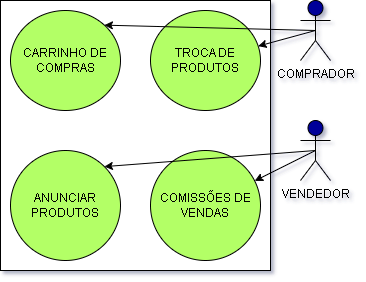
\includegraphics[scale=1.0]{Figuras/Casos de uso.drawio.png}
  \caption{Casos de Usos}
  \label{fig:partições}
\end{figure}

\section{\textbf{O que é um Produto Mínimo Viável (MVP)? \\ Explique o método proposto em Lean startup para construção e validação de MVPs}}
\label{sec:metodo}

MVP (Mínimo Produto Viável) serve para que você possa testar e validar se uma ideia é viável. Você entrega o mínimo a alguns usuários testarem, se tiver boa aceitação você pode refinar a ideia, senão, você descarta essa ideia. Muito comum em empresas de start-ups pois tem grande risco e maior incerteza sobre a ideia.

O método tem um ciclo de três passos: \textbf{construir, medir e aprender}. Abaixo será explicado cada um deles.

\begin{itemize}
    \item \textbf{Construir:} 
    Tem-se uma ideia de produto e então implementa-se um MVP para testá-la. 
    \item \textbf{Medir:} 
    o MVP é disponibilizado para uso por clientes com o intuito de coletar dados sobre a sua viabilidade.
    \item \textbf{Aprender:} 
    as métricas coletadas são analisadas e geram o que se denomina de aprendizado validado     \textit{(validated learning)}.
\end{itemize}

Ao final do ciclo pode-se fazer alguns ajustes e realizar o ciclo novamente, assim como, mudar o foco do produto ou simplesmente desistir da ideia. Mas se porvir a ter êxito, parte então para a construção de um produto mais sofisticado.

\section{\textbf{Explique as principais características do Design Sprint}}
\label{sec:design-sprint}

O \textbf{Design Sprint} tem geralmente a duração de cinco dias, ou seja, uma semana. Inicia-se em uma segunda-feira e termina na sexta-feira, tem que o objetivo de descobrir uma primeira solução para um problema rapidamente. 

Trabalham equipes pequenas e multidisciplinares, todos os representantes de todas as áreas envolvidas com o sistema devem participar e deve haver um tomador de decisões \textit{(líder)}.

Sobre os dias:
\begin{itemize}
    \item \textbf{Primeiro dia:} 
     entende-se e delimita-se o problema que se pretende resolver.
    \item \textbf{Segundo dia:} 
    possíveis alternativas de solução são propostas, de forma livre \textit{(divergência)}. 
    \item \textbf{Terceiro dia:}
    escolhe-se uma solução vencedora, dentre as possíveis alternativas \textit{(convergência)}. 
    \item \textbf{Quarto dia:} 
    implementa-se um protótipo, que pode ser simplesmente um conjunto de páginas HTML estáticas, sem qualquer código ou funcionalidade. 
    \item \textbf{Último dia:} 
    testa-se o protótipo com cinco clientes reais, com cada um deles usando o sistema em sessões individuais.
\end{itemize}

%\newpage
% ----------------------------------------------------------
% ELEMENTOS PÓS-TEXTUAIS
% ----------------------------------------------------------
%\postextual
% ----------------------------------------------------------
% Referências bibliográficas
% ----------------------------------------------------------
%\renewcommand{\bibsection}{%
%\section{\bibname}
%\bibmark
%\ifnobibintoc\else
%\phantomsection
%\addcontentsline{toc}{section}{\bibname}
%\fi
%\prebibhook}

%\bibliography{abntex2-modelo-references}

% ----------------------------------------------------------
% Apêndices
% ----------------------------------------------------------

% ---
% Inicia os apêndices
% ---
% \begin{apendicesenv}

% % ----------------------------------------------------------
% \section*{Apêndice A - Nome do Apêndice}
% \addcontentsline{toc}{section}{Apêndice A - Nome do Apêndice}
% % ----------------------------------------------------------

% \end{apendicesenv}
% % ---


% ----------------------------------------------------------
% Anexos
% ----------------------------------------------------------

% % ---
% % Inicia os anexos
% % ---
% \begin{anexosenv}

% % ---
% \section*{Anexo A - Nome do Anexo}
% \addcontentsline{toc}{section}{Anexo A - Nome do Anexo}
% % ---
% \end{anexosenv}


\end{document}
